\documentclass[12pt]{article}
\usepackage{amsmath, amsfonts, amsthm, amssymb}
\usepackage{fullpage}
\usepackage{enumerate}

% For figures
\usepackage{graphicx}
\usepackage{subcaption}

\usepackage{amsmath,amssymb}

\usepackage{hyperref}

%%%%%%%%%%%%%%%%%%%%CONTENT MACROS%%%%%%%%%%%%%%%%%%%%%%%%%
\renewcommand{\qed}{\quad \ensuremath{\blacksquare}}    % QED blacksquare
\newcommand{\inv}{^{-1}}                            % inverse operator
\newcommand{\sminus}{\backslash}                    % set minus
\newcommand{\N}{\mathbb{N}}                         % natural numbers
\newcommand{\R}{\mathbb{R}}                         % real numbers
\newcommand{\pow}{\mathcal{P}}                      % power set
\newcommand{\Se}{\mathcal{S}}                       % partition
\newcommand{\D}{\mathcal{D}}                        % partition
\newcommand{\e}{\varepsilon}                        % \varepsilon
\renewcommand{\d}{\delta}                           % \delta
\newcommand{\X}{\mathcal{X}}                        % X domain
\newcommand{\Y}{\mathcal{Y}}                        % Y domain
\newcommand{\Z}{\mathcal{Z}}                        % Z domain
\newcommand{\A}{\mathcal{A}}                        % sub-domain
\newcommand{\E}{\mathbb{E}}                         % expected value
\newcommand{\V}{\mathbb{V}}                         % variance
\newcommand{\pr}{\mathbb{P}}                        % probability
\newcommand{\dist}{\operatorname{dist}}             % distance operator
\newcommand{\acro}[1]{\textsc{\MakeLowercase{#1}}}
\newcommand{\ol}{\overline}
\newcommand{\wt}{\widetilde}
\renewcommand{\hat}{\widehat}
\newcommand{\defeq}{\vcentcolon=}
\newcommand{\eqdef}{=\vcentcolon}
\newcommand{\1}{\mathbbm{1}}
\newcommand{\C}{\text{Cov}}
%%%%%%%%%%%%%%%%%%%%%%%%%%%%%%%%%%%%%%%%%%%%%%%%%%%%%%%%%%%

\renewcommand{\thesubsection}{\arabic{subsection}}

\usepackage{natbib}
\usepackage[disable]{todonotes}

\begin{document}
\begin{center}
{\bf\Large 37-462/662 HW 02 Solutions}\\
\end{center}

\subsection{Problem 1 (Peter)}
\begin{enumerate}[(a)]
\item We can derive the result as follows
\begin{align*}
\text{df}(\hat y) &= \frac{1}{\sigma^2} \sum_{i=1}^n \C(\hat{y}_i,y_i) & \\
&= \frac{1}{\sigma^2} \text{tr}\left[\C(\hat{y},y)\right] & \C(\hat{y}_i,y_i)=\C(\hat{y},y)_{i,i}\\
&= \frac{1}{\sigma^2} \text{tr}\left[\C(Hy,y)\right] & \hat{y} = Hy\\
&= \frac{1}{\sigma^2} \text{tr}\left[H\C(y,y)\right] & \C(Ax,y) = A\C(x,y) \text{ in general}\\
&= \frac{1}{\sigma^2} \text{tr}\left[\sigma^2 H\right] & \C(y,y) = \V(y) = \sigma^2 I\\
&= \text{tr}(H) & \text{tr}(cX) = c\cdot\text{tr}(X)\\
&= \text{rank}(X) &\\
&= p &
\end{align*}
The last two lines follow from the fact that $H$ is a projection onto the column space of $X$. In general, the trace of a projection is equal to the dimension of the space onto which it projects. In this case the dimension is the rank of $X$, which is the number of predictors, $p$.
\item As shown in Homework 1 Problem 3, ridge regression is equivalent to linear regression with a modified hat matrix $H_{\text{ridge}} = X(X^TX+\lambda I)^{-1}X^T$. We can plug this in to the previous derivation:
\begin{align*}
\text{df}(\hat{y}_\text{ridge}) &= \text{tr}(H_\text{ridge}) \\
&=  \text{tr}\left[ X(X^TX+\lambda I)^{-1}X^T\right]
\end{align*}
Note that $H_\text{ridge}$ is not a projection matrix if $\lambda \neq 0$.
\end{enumerate}

\newpage
\subsection{Problem 2 (Shashank)}
\begin{enumerate}
\item[{\bf (a)}] {\bf (8 points)}

\begin{table}[h]
\centering
\begin{tabular}{|c|c|c|c|c|c|}
\hline
Regression Method           & OLS & \multicolumn{2}{|c|}{Lasso} & \multicolumn{2}{|c|}{Ridge} \\
\hline
$\lambda$                   & N/A & $\lambda_{min}$ & $\lambda_{1se}$ & $\lambda_{min}$ & $\lambda_{1se}$ \\
\hline
Prediction Error            & 1.76 & 1.14 & 1.13 & 1.46 & 1.46 \\
\hline
Cross-Validation Error      & N/A  & 1.26 & 1.45 & 1.61 & 1.80 \\
\hline
\end{tabular}
\caption{Prediction and cross-validation errors of various estimators.}
\label{tab:errs}
\end{table}

Table \ref{tab:errs} shows the relevant error values. Universally, lasso
performs, a followed by ridge, and then OLS. For lasso and ridge, cross
validation errors are consistently above prediction error. Figure
\ref{fig:cv_errs} plots cross-validation over $\lambda$ for both lasso and
ridge.

\begin{figure}[h!]
\centering
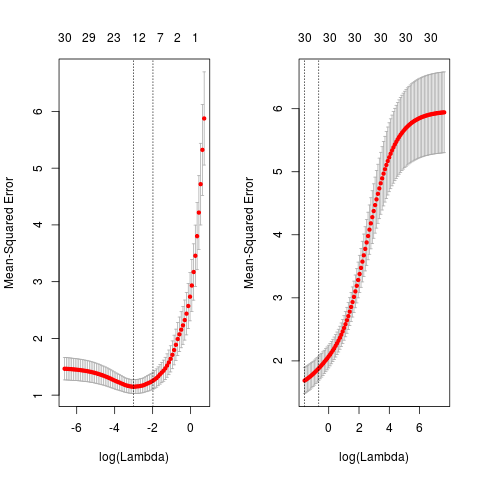
\includegraphics[width=0.8\linewidth]{CV_errors}
\vspace{-5mm}
\caption{Cross-validation error (with upper and lower standard deviation
curves) over $\lambda$, for lasso and ridge regression.}
\label{fig:cv_errs}
\end{figure}

\newpage
{\bf Grading:}
\begin{itemize}
\item 4 points for roughly correct prediction (OLS, lasso, and ridge,
$\lambda_{min}$ and $\lambda_{1se}$), cross-validation errors (lasso and ridge,
$\lambda_{min}$ and $\lambda_{1se}$)
\item 4 points for plots of cross-validation error over $\lambda$ (lasso and 
ridge, $\lambda_{min}$ and $\lambda_{1se}$)
\end{itemize}

\item[{\bf (b)}] {\bf (6 points)}
$\hat \beta^{lasso}_{min}$ had 11 nonzero components,
$\hat \beta^{lasso}_{1se}$ had 7 nonzero coefficients, and each
$\hat \beta^{lasso}_{min}$ and $\hat \beta^{lasso}_{1se}$ had all 30
coefficients nonzero, as we expect for ridge regression. Thus the costs for the
$\lambda_{min}$ lasso prediction, the $\lambda_{1se}$ lasso prediction, and
each ridge regression prediction are $\$700$, $\$1,100$, and $\$3,000$,
respectively. Since the $\lambda_{1se}$ estimate has the lowest prediction
error and cost, it seems to be the most cost effective. In comparison, the
$\lambda_{min}$ and both ridge predictors are each a waste of money, as they
have higher error and are more expensive to evaluate.

{\bf Grading:}
\begin{itemize}
\item 4 points for roughly correct costs of evaluating each estimator (lasso
and ridge, $\lambda_{min}$ and $\lambda_{1se}$)
\item 2 points for commenting on these costs
\end{itemize}

\item[{\bf (c)}] {\bf (6 points)}
Looking at the coefficients in Table \ref{tab:3coeffs}, we see that the lasso
zeros out two of the three coefficients, while all ridge coefficients are
nonzero. This is consistent with the fact that we know lasso promotes sparsity,
whereas ridge regression only shrinks large coefficients. As discussed in part
(b), if nonzero coefficients are expensive, lasso gives the best behavior:
minimizing cost while maximizing predictive power.

\begin{table}[h]
\centering
\begin{tabular}{|l|c|c|c|}
\hline
Regression Method       & $\hat\beta_1$ & $\hat\beta_2$ & $\hat\beta_3$ \\
\hline
OLS                     & -0.10         & 2.43          & -0.45         \\
\hline
Lasso, $\lambda_{min}$  & 0.00          & 1.91          & 0.00          \\
\hline
Lasso, $\lambda_{1se}$  & 0.00          & 1.80          & 0.00          \\
\hline
Ridge, $\lambda_{min}$  & 0.20          & 1.70          & -0.06         \\
\hline
Ridge, $\lambda_{1se}$  & 0.31          & 1.32          & 0.14          \\
\hline
\end{tabular}
\caption{First three estimated coefficients under each model.}
\label{tab:3coeffs}
\end{table}

{\bf Grading:}
\begin{itemize}
\item 3 points for discussing how lasso and ridge ($\lambda_{min}$ and
$\lambda_{1se}$) handle correlated covariates
\item 3 points for discussing which is better for minimizing evaluation costs
\end{itemize}

{\bf Notes about correlated predictors:} Several students claimed that the
(ridge) penalty $\lambda \|\beta\|_2^2$ shrinks all the coefficients. However,
looking at the coefficients for OLS in Table \ref{tab:3coeffs}, we see that, as
$\lambda$ increases, coefficients can actually move further from zero as well
as switch sign. This is because ridge penalizes large coefficients much more
than small coefficients, forcing large coefficients to shrink, without
controlling small coefficients much.

Specifically, by shrinking large coefficients, ridge increases the squared loss
$\|y - X\beta\|$. Increasing the coefficients of correlated variables with
small coefficients counteracts this. This means that, for highly correlated
variables, rather than forcing coefficients to be zero, the ridge penalty
forces coefficients to have similar magnitude.

Most students correctly observed that lasso tends to zero the smallest
coefficients of correlated predictors.
Some students also concluded that lasso handles correlated coefficients better
than ridge regression. This is true for this problem, but shouldn't be taken as
a general rule. For pure prediction, we don't care about the values of
coefficients. But suppose we were actually interested in learning which genes
might be related to the outcome (immune response). Since highly correlated
variables contain very similar information, we would want their coefficients to
be similar, as in ridge regression. Thus, when thinking about which penalty to
use, the end goal has to be considered, alongside error and sparsity.

Finally, if we want both sparsity and interpretability with correlated
variables, a natural idea might be to use both ridge and lasso penalties:
$\lambda_1 \|\beta\|_1 + \lambda_2 \|\beta\|_2^2$. This is the basis of another
linear regression approach, the \emph{elastic net} (which is what
\texttt{glmnet} does for $\alpha \in (0,1)$).
\end{enumerate}

\newpage
\subsection{Problem 3 (Peter)}
\begin{enumerate}[(a)]
\item The following plot shows fitted curves selected by 10-fold cross validation.
\begin{center}
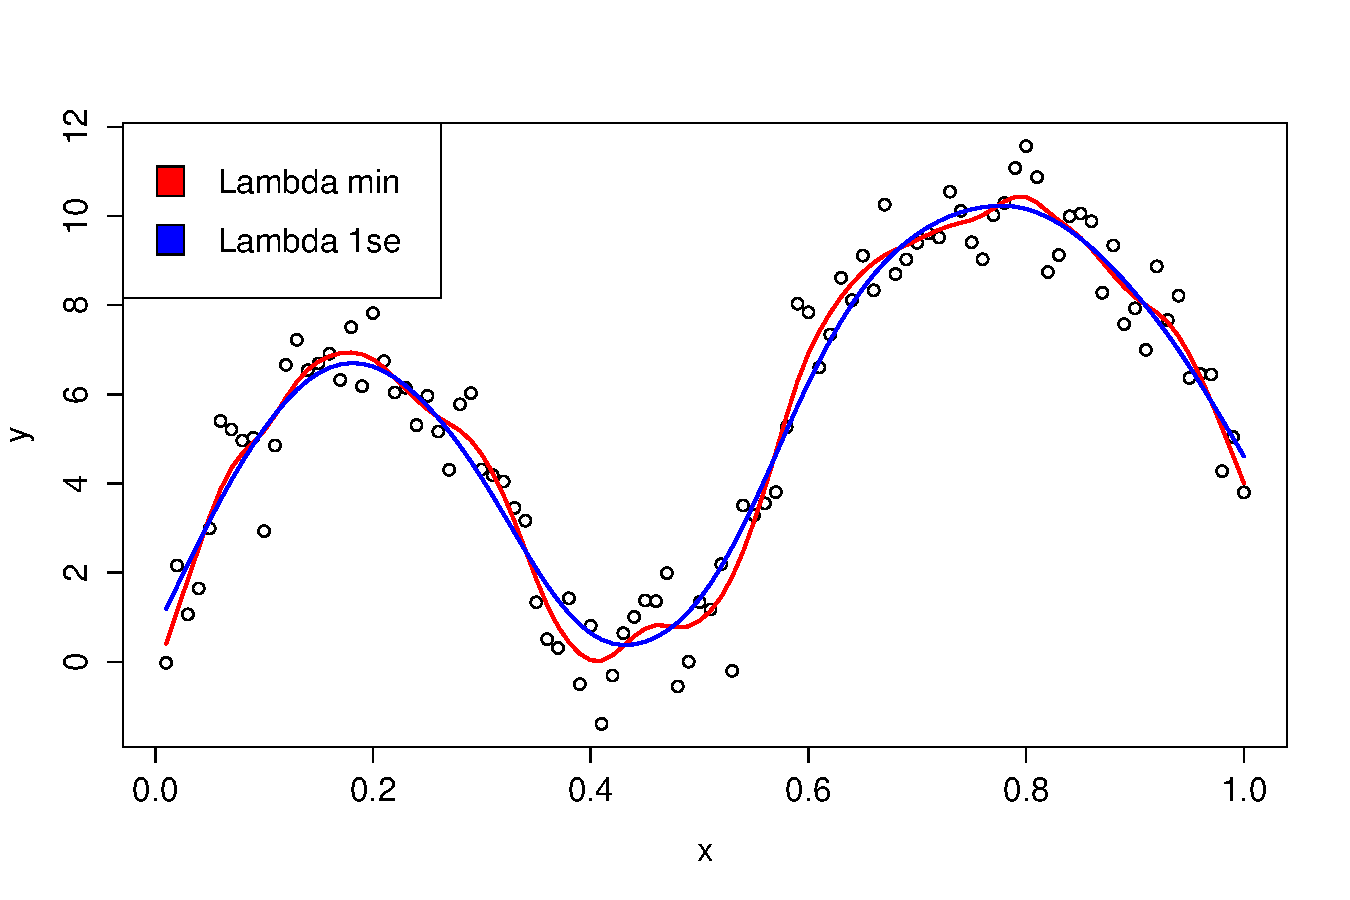
\includegraphics[width=5in]{prob3_a_1.pdf}
\end{center}
The curves are very similar, but the model with $\lambda_{1\text{se}}$ looks like it fits better. The one standard error rule creates a much smoother curve.
\item The following plot shows curves fitted with 5-fold cross validation, with each fold sequential rather than using alternating points.
\begin{center}
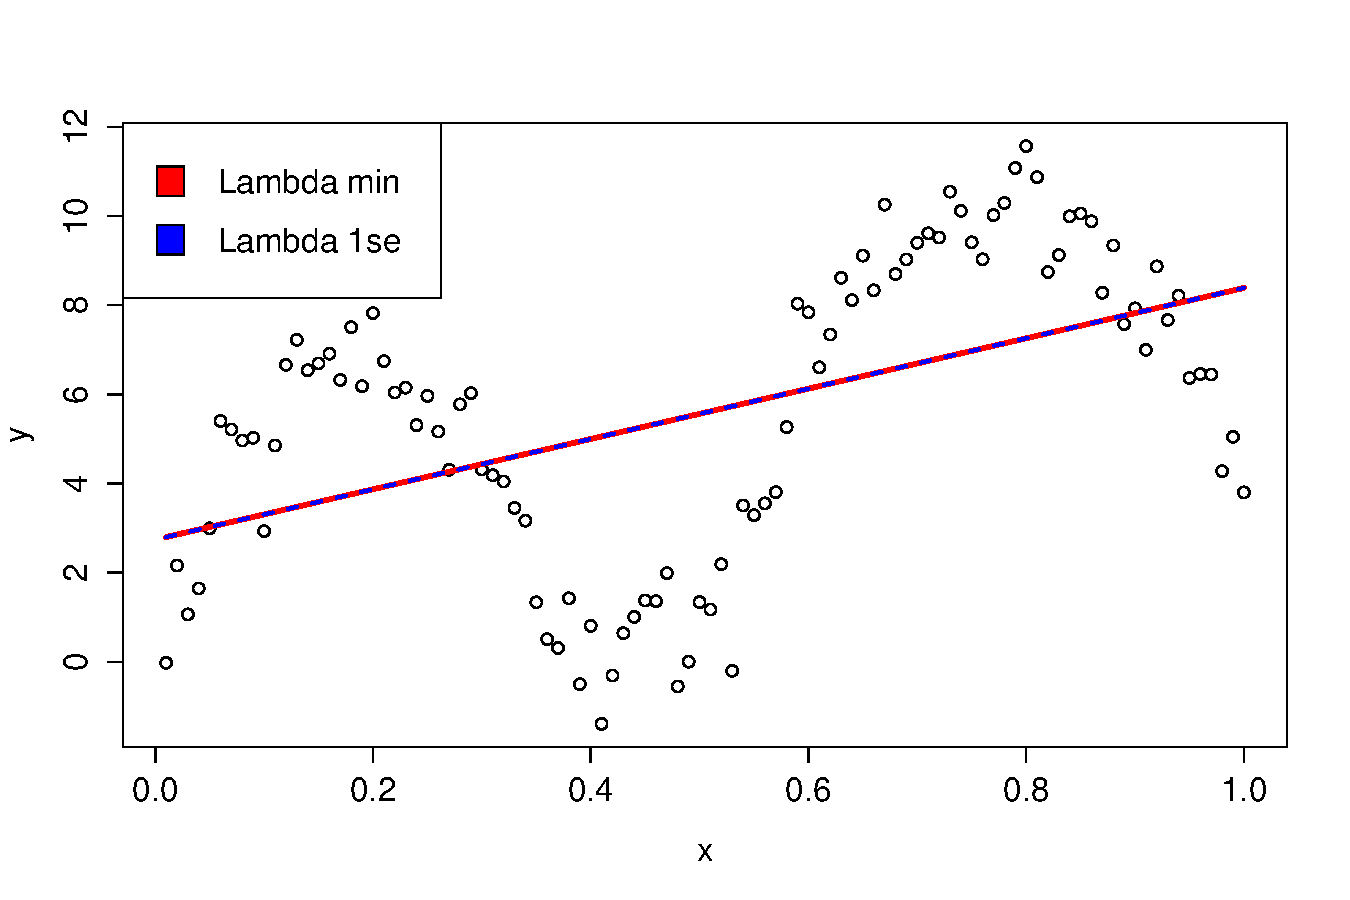
\includegraphics[width=5in]{prob3_b_1.pdf}
\end{center}
In this case cross validation chooses the simplest possible model. This is likely because models with more degrees of freedom extrapolate poorly on excluded segments of the data.
Alternatively, if we use 10 fold CV we get the following plot.
\begin{center}
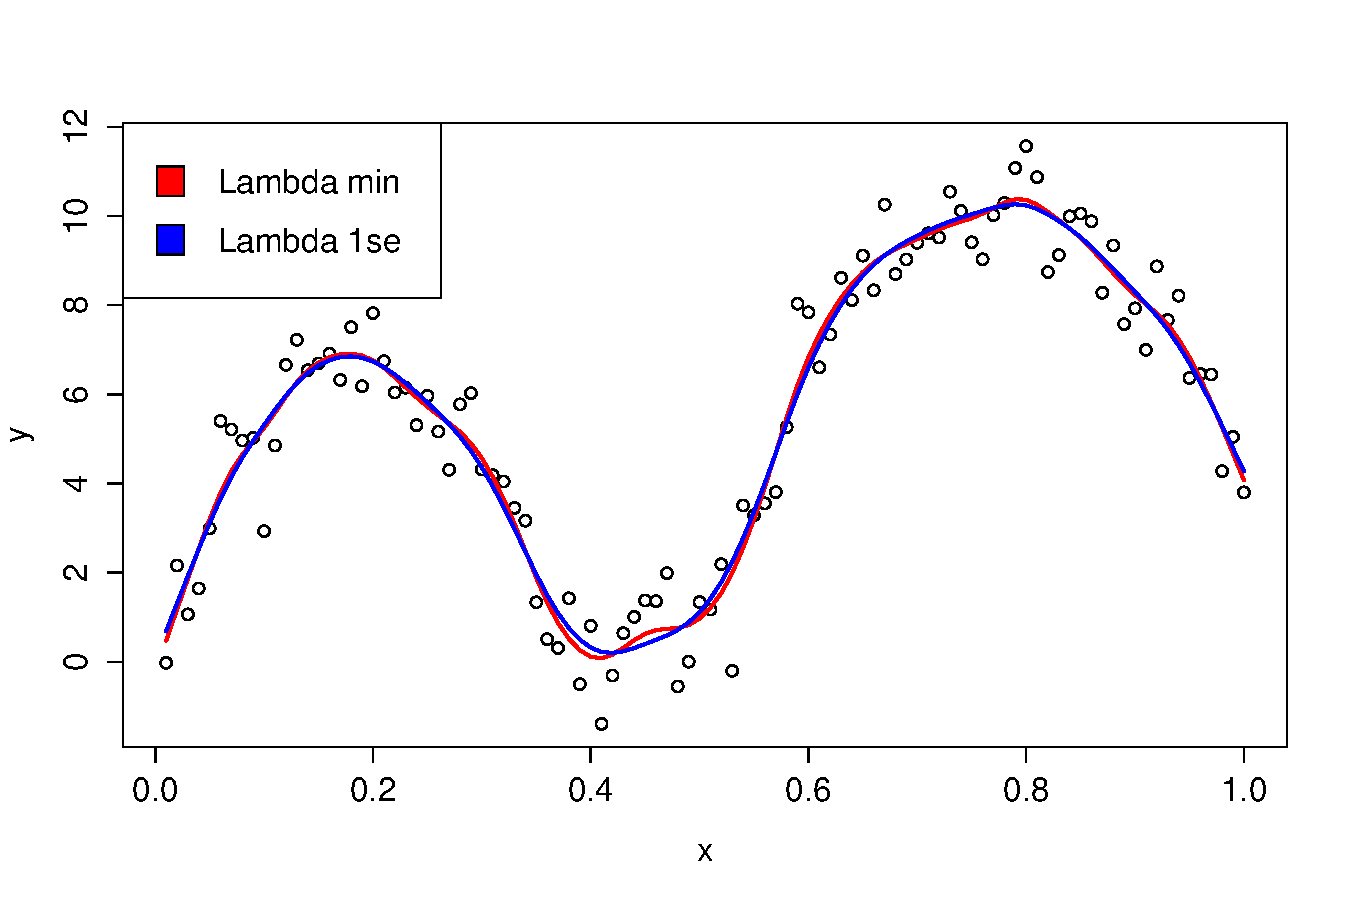
\includegraphics[width=5in]{prob3_b_2.pdf}
\end{center}
\item The following plot compares the result of leave-one-out cross validation with the shortcut formula.
\begin{center}
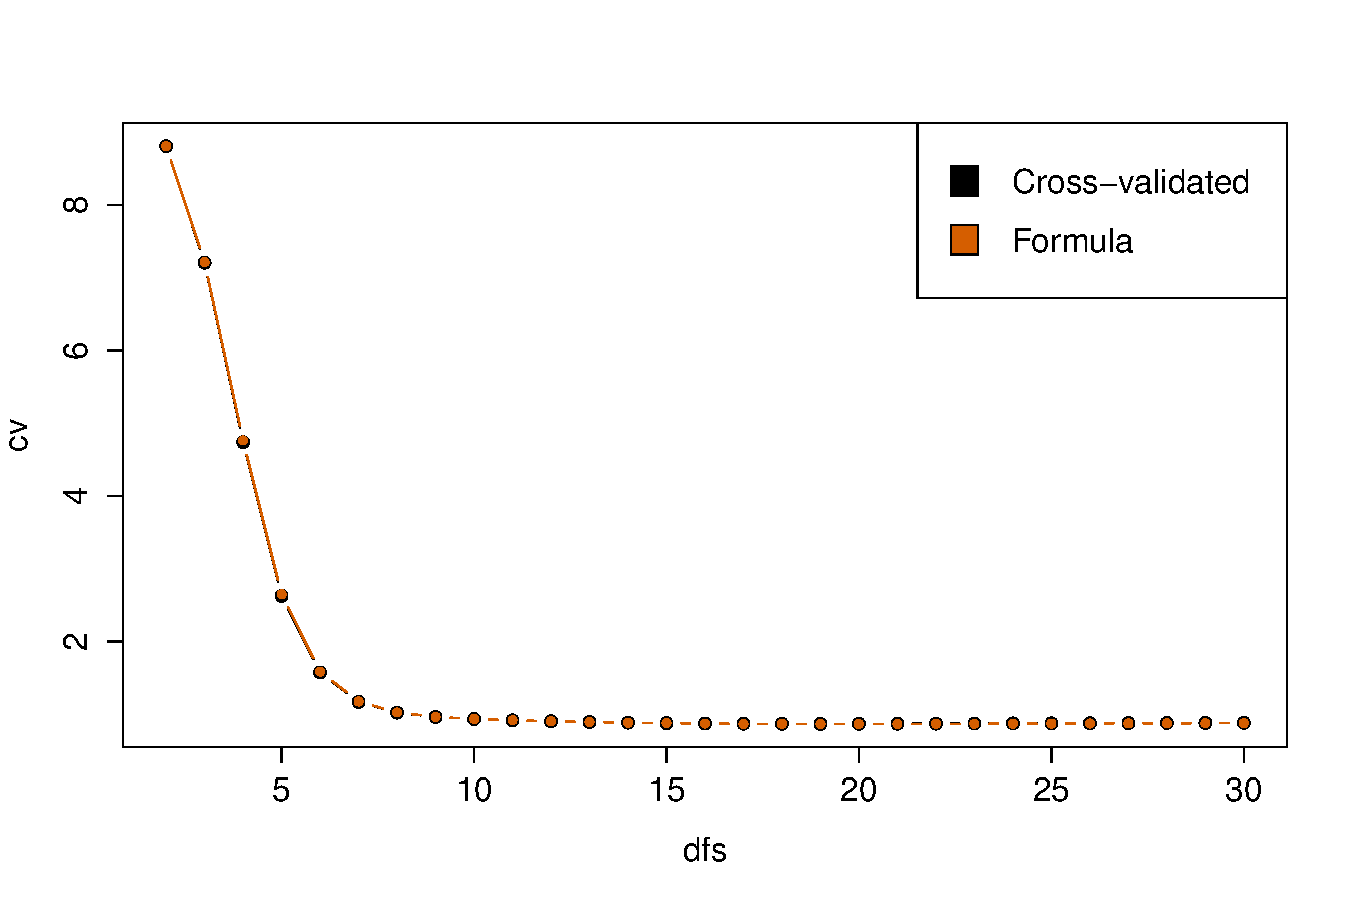
\includegraphics[width=5in]{prob3_c_1.pdf}
\end{center}
The plot shows that the values are nearly the same over the various degrees of freedom, as should be expected from Problem 4.
\end{enumerate}
\subsection{Problem 4 (Shashank)}
\begin{enumerate}
\item[{\bf (a)}] {\bf (4 points)} Let $\vec e_i \in \R^n$ denote the $i^{th}$
canonical basis (column) vector:
\[(e_i)_j = \left\{
        \begin{array}{ll}
            1 & \mbox{ if } i = j   \\
            0 & \mbox{ else }
        \end{array}
    \right.
\]
For any matrix $A$, $e_i^TA$ is the $i^{th}$ row of $A$ and $Ae_i$ is the
$i^{th}$ column of $A$. Thus,
\[S_{i,i}
    = e_i^T S e_i
    = (e_i^T X) (X^T X)\inv (X^T e_i)
    = x_i^T (X^T X)\inv x_i.
\]
By the usual linear regression prediction formula,
\[f^{-i}(x_i) = x_i^T \hat\beta_{-i} = x_i^T (Z^T Z)\inv Z^T y_{-i}.\]
Also, since
\[X^T X
    = 
    \begin{bmatrix}
        x_1 \cdots x_n
    \end{bmatrix}
    \begin{bmatrix}
        x_1     \\
        \vdots  \\
        x_n
    \end{bmatrix}
    = \sum_{j = 1}^n x_j x_j^T.\]
\[\quad \mbox{ and } \quad
Z^T Z
    = 
    \begin{bmatrix}
        x_1 \cdots x_{i - 1} \;\; x_{i + 1} \cdots x_n
    \end{bmatrix}
    \begin{bmatrix}
        x_1         \\
        \vdots      \\
        x_{i - 1}   \\
        x_{i + 1}   \\
        \vdots      \\
        x_n
    \end{bmatrix}
    = \sum_{j \neq i} x_j x_j^T,\]
Thus, $X^T X = Z^T Z + x_i x_i^T$. Finally,
\[X^T y
    = \sum_{j = 1}^n y_j x_j
    = \sum_{j \neq i} y_j x_j + x_i y_i
    = Z^T y_{-i} + x_i y_i. \qed\]

\item[{\bf (b)}] {\bf (10 points)}
For convenience, define $A := x_i^T (X^T X)\inv$. By part (a) and the
Sherman-Morrison update formula (with $u = -x_i,v = x_i$),
\begin{align*}
(Z^T Z)\inv
    = (X^T X - x_i x_i^T)\inv
 &  = (X^T X)\inv + \frac{(X^T X)\inv x_i x_i^T (X^T X)\inv}
                         {1 - x_i^T (X^T X)\inv x_i}    \\
 &  = \frac{(1 - S_{i,i}) (X^T X)\inv + A^T A}{1 - S_{i,i}}.
\end{align*}

Thus, using part (a) again, since $\hat f(x_i) = A X^T y$ and
$S_{i,i} = A x_i$,
\begin{align*}
\hat f^{-i}(x_i)
 &  = x_i^T (Z^T Z)\inv Z^T y_{-i}
    = x_i^T (Z^T Z)\inv \left( X^T y - x_i y_i \right)  \\
 &  = x_i^T \left( \frac{(1 - S_{i,i})(X^T X)\inv + A^T A}{1 - S_{i,i}} \right)
                                            \left( X^T y - x_i y_i \right)  \\
 &  = \frac{(1 - S_{i,i})\hat f(x_i) + S_{i,i} \hat f(x_i)
            - (1 - S_{i,i})S_{i,i} y_i - S_{i,i} S_{i,i} y_i}{1 - S_{i,i}}
    = \frac{\hat f(x_i) - S_{i,i} y_i}{1 - S_{i,i}}.
\end{align*}
Thus,
\[y_i - f^{-i}(x_i)
    = y_i - \frac{\hat f(x_i) - S_{i,i} y_i}{1 - S_{i,i}}
    = \frac{y_i(1 - S_{i,i}) + S_{i,i} y_i - \hat f(x_i)}{1 - S_{i,i}}
    = \frac{y_i - \hat f(x_i)}{1 - S_{i,i}}. \qed\]

\item[{\bf (c)}] {\bf (6 points)} In Problem 3(a) of Homework 1, we showed
that, for any tuning parameter $\lambda \geq 0$ and $x \in \R^p$, the ridge
regression estimate $\hat f(x)$ is the same as the linear regression estimate
computed from the modifed response vector
$\wt y = \begin{bmatrix} y \\ 0_p \end{bmatrix} \in \R^{n + p}$
and the covariate matrix
$\wt X = \begin{bmatrix} X \\
    \sqrt\lambda I_p \end{bmatrix} \in \R^{(n + p) \times p}$.
Note that,
\[\wt X^T \wt X
    = \begin{bmatrix} X \\ \sqrt\lambda I_p \end{bmatrix}^T
        \begin{bmatrix} X \\ \sqrt\lambda I_p \end{bmatrix}
    = X^T X + \left( \sqrt\lambda I_p \right)^T \left( \sqrt\lambda I_p \right)
    = X^T X + \lambda I_p,\]
and so, for the modified hat matrix $S = \wt X (\wt X^T \wt X)\inv \wt X^T$,
\[S_{i,i}
    = e_i^T S e_i
    = (e_i^T \wt X) \left( X^T X + \lambda I_p \right)\inv \wt X^T e_i
    = x_i^T \left( X^T X + \lambda I_p \right)\inv x_i.
\]
Thus, part (b) gives
\[y_i - f^{-i}(x_i) = \frac{y_i - \hat f(x_i)}{1 - S_{i,i}}. \qed\]

{\bf Note:} Parts (a) and (b) were relatively straightforward. For part (c),
many students simply repeated the proof of part (b). This is unnecessary,
because we showed in Homework 1 that ridge regression is a special case of
linear regression, and so we can actually apply the result of part (b)
directly. What remains is to show that the diagonal entries of
$X (X^T X + \lambda I_p)\inv X^T$ are the same as the $S_{i,i}$ values (the
diagonal entries of the hat matrix) used in part (b).
\end{enumerate}

\newpage
\subsection{Problem 5 (Peter)}
\begin{enumerate}[(a)]
\item The dimension of the original feature space is 256, while dimension of the transformed space is 2. The following plot shows the data in the transformed space:
\begin{center}
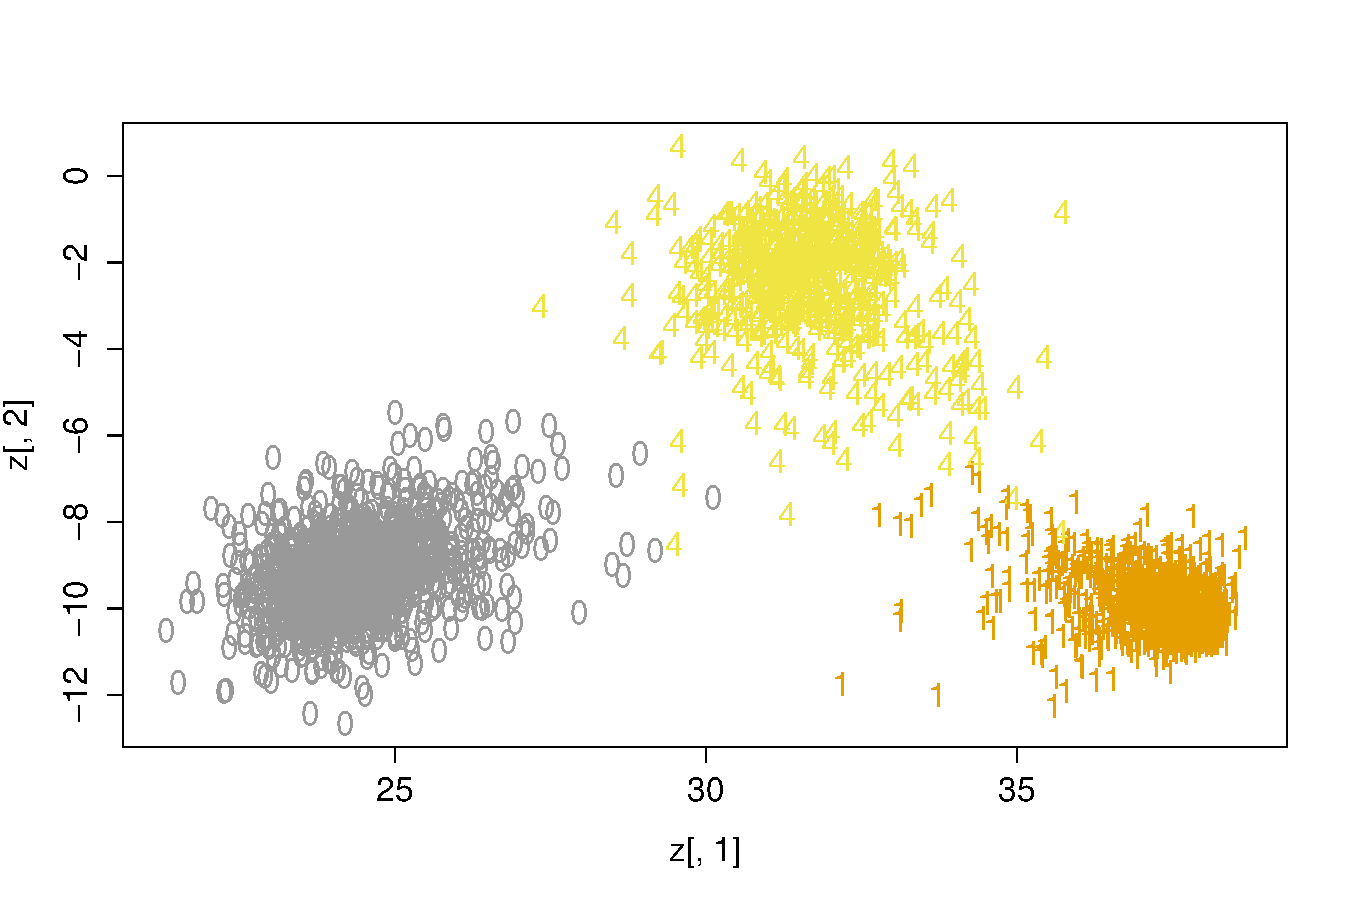
\includegraphics[width=3.5in]{prob5_a_1.pdf}
\end{center}

\stepcounter{enumii}
\item The misclassification rate is $2.07\%$. See code.
\item We replot the data with misclassified points labeled.

\begin{center}
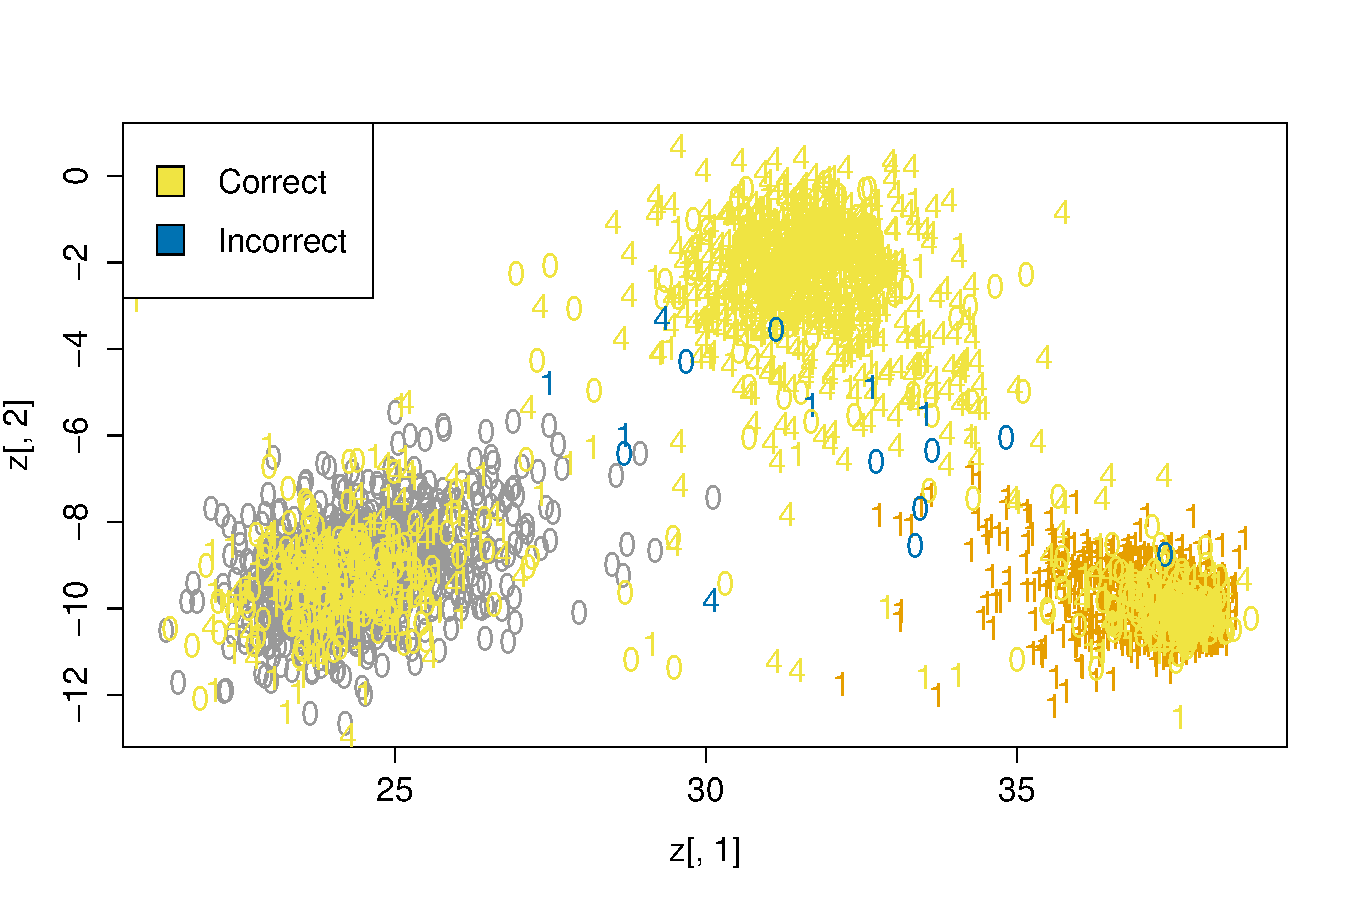
\includegraphics[width=3.5in]{prob5_d_1.pdf}
\end{center}
Some of the misclassified points are shown below.
\begin{center}
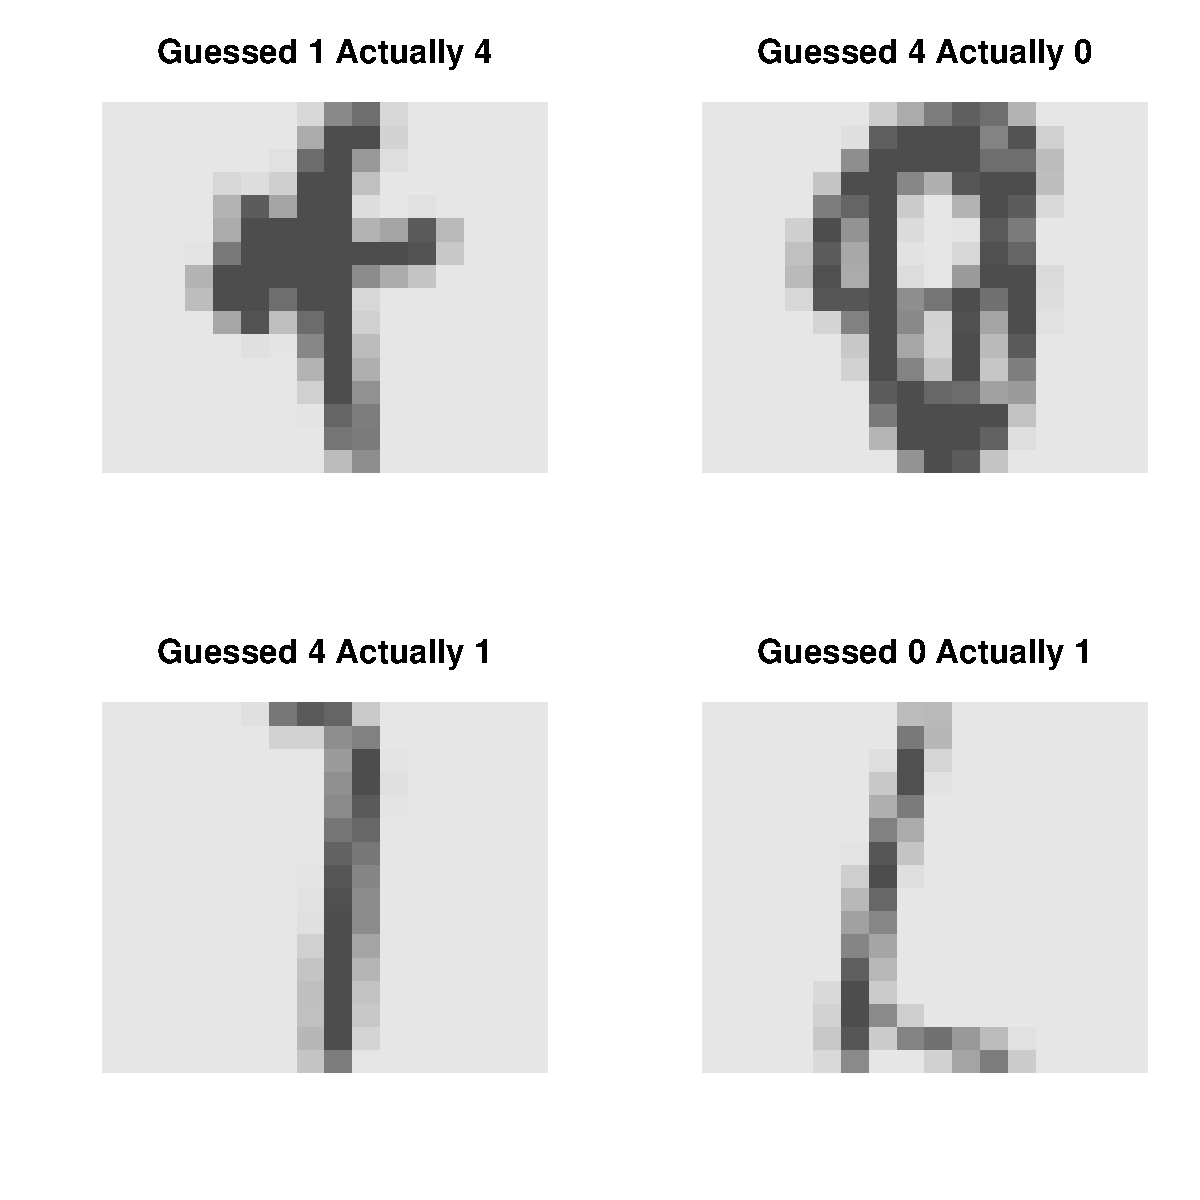
\includegraphics[width=3.5in]{prob5_d_2.pdf}
\end{center}
Going clockwise from the top left, the first and fourth misclassified examples are easy to classify by eye so you would hope the algorithm could correctly predict them. The second and third misclassified examples, on the other hand, are very ambiguous.
\end{enumerate}

\newpage
\subsection{Code Appendix}
\label{sec:code}
\begin{verbatim}
load("hw2problem2.Rdata")
library(glmnet)
set.seed(0) # just to standardize our solutions

#### PROBLEM 2 ####
#### Part (a) ####
# Least squares
fit_ls = lm(y_train ~ X_train)
yhat_ls = X_test%*%fit_ls$coefficients[-1] + fit_ls$coefficients[1]
pe_ls = mean((yhat_ls - y_test)^2) # compute least squares MSE

# Perform fitting
fit_lasso = glmnet(X_train,y_train,family='gaussian',alpha=1)
fit_ridge = glmnet(X_train,y_train,family='gaussian',alpha=0)

# Perform cross-validation
cv_lasso = cv.glmnet(X_train,y_train,family='gaussian',alpha=1)
cv_ridge = cv.glmnet(X_train,y_train,family='gaussian',alpha=0)

# Extract indices of relevant lambdas
lasso_idx_min = which(cv_lasso$lambda==cv_lasso$lambda.min)
lasso_idx_1se = which(cv_lasso$lambda==cv_lasso$lambda.1se)
ridge_idx_min = which(cv_ridge$lambda==cv_ridge$lambda.min)
ridge_idx_1se = which(cv_ridge$lambda==cv_ridge$lambda.1se)

# Perform prediction on test data
yhat_lasso_min = predict(cv_lasso,newx=X_test,s=cv_lasso$lambda[lasso_idx_min])
yhat_lasso_1se = predict(cv_lasso,newx=X_test,s=cv_lasso$lambda[lasso_idx_1se])
yhat_ridge_min = predict(cv_ridge,newx=X_test,s=cv_ridge$lambda[ridge_idx_min])
yhat_ridge_1se = predict(cv_ridge,newx=X_test,s=cv_ridge$lambda[ridge_idx_1se])

# Compute prediction errors on test data
pe_lasso_min = mean((yhat_lasso_min - y_test)^2)
pe_lasso_1se = mean((yhat_lasso_1se - y_test)^2)
pe_ridge_min = mean((yhat_ridge_min - y_test)^2)
pe_ridge_1se = mean((yhat_ridge_1se - y_test)^2)

# Extract relevant cross-validation errors
cvm_lasso_min = cv_lasso$cvm[lasso_idx_min]
cvm_lasso_1se = cv_lasso$cvm[lasso_idx_1se]
cvm_ridge_min = cv_ridge$cvm[ridge_idx_min]
cvm_ridge_1se = cv_ridge$cvm[ridge_idx_1se]

# Print relevant error values
cat("Least Squares Prediction Error: ", pe_ls, "\n\n")
print('Lasso Prediction Errors:')
cat("lambda.min: ", pe_lasso_min, "  lambda.1se: ", pe_lasso_1se, "\n\n")
print('Ridge Prediction Errors:')
cat("lambda.min: ", pe_ridge_min, "  lambda.1se: ", pe_ridge_1se, "\n\n")
print('Lasso Cross-Validation Errors:')
cat("lambda.min: ", cvm_lasso_min, "  lambda.1se: ", cvm_lasso_1se, "\n\n")
print('Ridge Cross-Validation Errors:')
cat("lambda.min: ", cvm_ridge_min, "  lambda.1se: ", cvm_ridge_1se, "\n\n")

# Plot cross-validation error over lambdas
par(mfrow=c(1,2))
plot(cv_lasso)
plot(cv_ridge)

#### Part (b) ####
# Compute number of nonzero components of beta
nnz_lasso_min = sum(fit_lasso$beta[,lasso_idx_min] != 0)
nnz_lasso_1se = sum(fit_lasso$beta[,lasso_idx_1se] != 0)
nnz_ridge_min = sum(fit_ridge$beta[,ridge_idx_min] != 0)
nnz_ridge_1se = sum(fit_ridge$beta[,ridge_idx_1se] != 0)

# Print number of nonzero beta components in each model
print('Lasso Nonzeros:')
cat("lambda.min: ", nnz_lasso_min, "  lambda.1se: ", nnz_lasso_1se, "\n\n")
print('Ridge Nonzeros:')
cat("lambda.min: ", nnz_ridge_min, "  lambda.1se: ", nnz_ridge_1se, "\n\n")

#### Part (c) ####
# Print first 3 beta coefficients in each model
print('First 3 Beta Coefficients under Lasso, lambda.min:')
print(fit_lasso$beta[1:3,lasso_idx_min])
print('First 3 Beta Coefficients under Lasso, lambda.1se:')
print(fit_lasso$beta[1:3,lasso_idx_1se])
print('First 3 Beta Coefficients under Ridge, lambda.min:')
print(fit_ridge$beta[1:3,ridge_idx_min])
print('First 3 Beta Coefficients under Ridge, lambda.1se:')
print(fit_ridge$beta[1:3,ridge_idx_1se])

#### PROBLEM 3 ####
#Load the data (appears in variable y in the workspace)
load(file="splines.Rdata")
#100 points uniformly spaced from 0 to 1
n = 100
x = 1:n/n

K = 5 #Number of folds (5 or 10 for parts A and B, 100 for part C)

#Generate a list with index vectors for each fold
folds = vector(mode="list",length=K)
for (k in 1:K) {
  #Choose folds to alternate sequentially
  
  #Folds for parts A and C
  #folds[[k]] = seq(k,n,by=K) 
  
  #Folds for part B:
  #folds[[k]] = ((k-1)*(n/K)+1):(k*n/K)
}

dfs = 2:30#Range of degrees of freedom (similar to lambda)
ndfs = length(dfs)

#Store the error at every point for every degree of freedom.
#This makes sense, because each point only gets estimated once,
#when its fold is held out
errs = matrix(0,n,ndfs)

#Run CV
for (k in 1:K) {
  #Build the test and training data sets corresponding to the kth fold
  #Variables ending in .tr are for training
  #Variables ending in .val are for validation (the held out fold)
  i.tr = unlist(folds[-k])
  i.val = folds[[k]]
  x.tr = x[i.tr]    
  y.tr = y[i.tr]   
  x.val = x[i.val] 
  y.val = y[i.val]
  
  #Fit and evaluate a spline on this fold at each degree of freedom being considered
  for (j in 1:ndfs) {
    a = smooth.spline(x.tr,y.tr,df=dfs[j])
    yhat = predict(a,x=x.val)$y
    errs[i.val,j] = (yhat-y.val)^2
  }
}

predict(a,x=x.val)$y
predict(a,newx=x.val)$y

#Average cv error across folds for each degree of freedom
cv = colMeans(errs)

#Compute the standard error across the folds for the cv estimate
#Stores the average error for each fold (so we can take variance)
errs0 = matrix(0,K,ndfs)
for (k in 1:K) {
  # if using folds < n
  # errs0[k,] = colMeans(errs[folds[[k]],])
  # if using LOOCV
  # errs0[k,] = colMeans(matrix(errs[folds[[k]],],nrow=1))
}
se = apply(errs0,2,sd)/sqrt(K)

# Usual rule
i1 = which.min(cv)
# One standard error rule---note the min!
i2 = min(which(cv<=cv[i1]+se[i1]))

#Plot the cv curve
plot(dfs,cv,type="l",ylim=range(c(cv-se,cv+se)))
points(dfs,cv,pch=20)
lines(dfs,cv-se,lty=3)
lines(dfs,cv+se,lty=3)
abline(v=dfs[i1],col="red",lty=2)
abline(v=dfs[i2],col="blue",lty=2)
legend('top',fill=c('red','blue'),legend=c("Lambda min","Lambda 1se"))

#Form estimates for lambda_min and lambda_1se
yhat1 = smooth.spline(x,y,df=dfs[i1])$y
yhat2 = smooth.spline(x,y,df=dfs[i2])$y

#Plot splines for lambda_min and lambda_1se
plot(x,y)
lines(x,yhat1,col="red",lwd=2)
lines(x,yhat2,col="blue",lwd=2)
legend('topleft',fill=c('red','blue'),legend=c("Lambda min","Lambda 1se"))

#Part C: You can eventually put your code down here to get the S_ii elements
#and compare your LOOCV to the equation from the homework

#Computing LOOCV using the closed form formula (Part C)
closed_form = numeric(ndfs)
for(j in 1:ndfs){
  a = smooth.spline(x,y,df=dfs[j])
  yhat = predict(a,x=x)$y
  Sii = a$lev
  closed_form[j] = mean(((y-yhat)/(1-Sii))^2)
}
plot(dfs,cv,type='b',pch=19)
lines(dfs,closed_form,type='b',col="#D55E00",pch=20)
legend('topright',legend=c("Cross-validated","Formula"),fill=c("black","#D55E00"))
#The two match quite closely!























#### PROBLEM 5 ####
load('zip.014.Rdata')

#A
library(MASS)
a = lda(x.014.tr,y.014.tr)
z = x.014.tr%*%a$scaling

#original dimension
ncol(x.014.tr)
#new dimension
ncol(z)

cbPalette <- c("#999999", "#E69F00", "#56B4E9", "#009E73", "#F0E442", "#0072B2", "#D55E00", "#CC79A7")#I like these colors more
plot(z[,1],z[,2],pch=as.character(y.014.tr),col=cbPalette[y.014.tr+1])

yhat = predict(a,newdata = x.014.te)$class
#Misclassification rate
mean(yhat!=y.014.te)

#Transform the test points into the same space as the training points
z.te = x.014.te%*%a$scaling

plot(z[,1],z[,2],pch=as.character(y.014.tr),col=cbPalette[y.014.tr+1])
points(z.te[,1],z.te[,2],pch=as.character(y.014.tr),col=cbPalette[5+(yhat!=y.014.te)])
legend('topleft',legend=c("Correct","Incorrect"),fill=c("#F0E442", "#0072B2"))

plot.digit = function(x,zlim=c(-1,1)) {
  cols = gray.colors(100)[100:1]
  image(matrix(x,nrow=16)[,16:1],col=cols,
        zlim=zlim,axes=FALSE)  
}
idx = which(yhat != y.014.te)
par(mfrow=c(2,2))
for(i in 1:4){
  plot.digit(x.014.te[idx[i],])
  title(paste("Guessed",yhat[idx[i]],"Actually",y.014.te[idx[i]]))
}
\end{verbatim}

%{\small
%\bibliography{biblio}
%%\bibliographystyle{icml2014}
%\bibliographystyle{plain}
%}
\end{document}
